\documentclass{beamer}

\usetheme{simple}

\usepackage{scalerel,xparse}
\usepackage{lmodern}
\usepackage[scale=2]{ccicons}
\usepackage{ulem}
\usepackage{tikz}
\usetikzlibrary{positioning,calc,automata}
\usepackage{algorithm}
\usepackage{algorithmic}
\usepackage{caption}
\usepackage{listings}

% Watermark background (simple theme)
\setlength{\parindent}{0cm}
\setwatermark{
\includegraphics[height=8cm]{img/chungus.png}}


\title{CSC363H5 Tutorial 2}
\subtitle{I hope you can read the following Greek letters: $\Sigma, \Gamma, \delta$}
\date{\today}
\author{Paul ``sushi{\textunderscore}enjoyer'' Zhang}
\institute{University of Chungi}


\NewDocumentCommand\emojisushi{}{
    
\includegraphics{img/1f363.png}
}
\NewDocumentCommand\emojifish{}{
    
\includegraphics{img/1f41f.png}
}
\NewDocumentCommand\emojirice{}{
    
\includegraphics{img/1f35a.png}
}
\NewDocumentCommand\emojijoy{}{

    
\includegraphics{img/1f602.png}
}
\NewDocumentCommand\emojicarrot{}{
    
\includegraphics[scale=0.04]{img/1f955.png}
}

\begin{document}

\maketitle

\begin{frame}{Learning objectives this tutorial}
By the end of this tutorial, you should...
\begin{itemize}
\item Have an informal idea of the formal definition of a Turing machine.
\item Be able to build a very basic Turing machine that adds 1 to a number. Then question why anything in this course is applicable to actual programming, as you can just write \texttt{chungus += 1} instead.
\item Understand the Turing machine definition of ``decidable'' and ``listable'', and take without proof that these definitions are equivalent to the definitions in class.
\item Have a brief understanding of the \textit{halting problem} and why it is a listable but undecidable language.
\item Question why all the G*del computable material was necessary.
\end{itemize}
\end{frame}

\begin{frame}{helo!}
\texttt{helo{\textunderscore}fish.jpg} is feeling sad today :((((
\begin{figure}

\includegraphics[scale=0.2]{img/helo_fish_sad.jpg}
\end{figure}
Why is she sad? Because life really do be like that. 

Also she is sad because G*del computable is too much math.

  \begin{columns}
    \column{.5\textwidth}
    Anyway, if you want to make \texttt{helo{\textunderscore}fish.jpg} feel better, please respond to her greetings by saying ``helo'', and then post your credit card number(s) in the chat.

    \column{.5\textwidth}
      \begin{block}{Protip...}
         If \texttt{helo{\textunderscore}fish.jpg} does not appear in your dreams, please find a therapist who can perform Jungian analysis for you.
      \end{block}
  \end{columns}
  
\end{frame}

\begin{frame}{sad \texttt{helo{\textunderscore}fish.jpg} wants you to learn about Turing machines.}

But what really is a Turing machine? 

\begin{figure}[h]
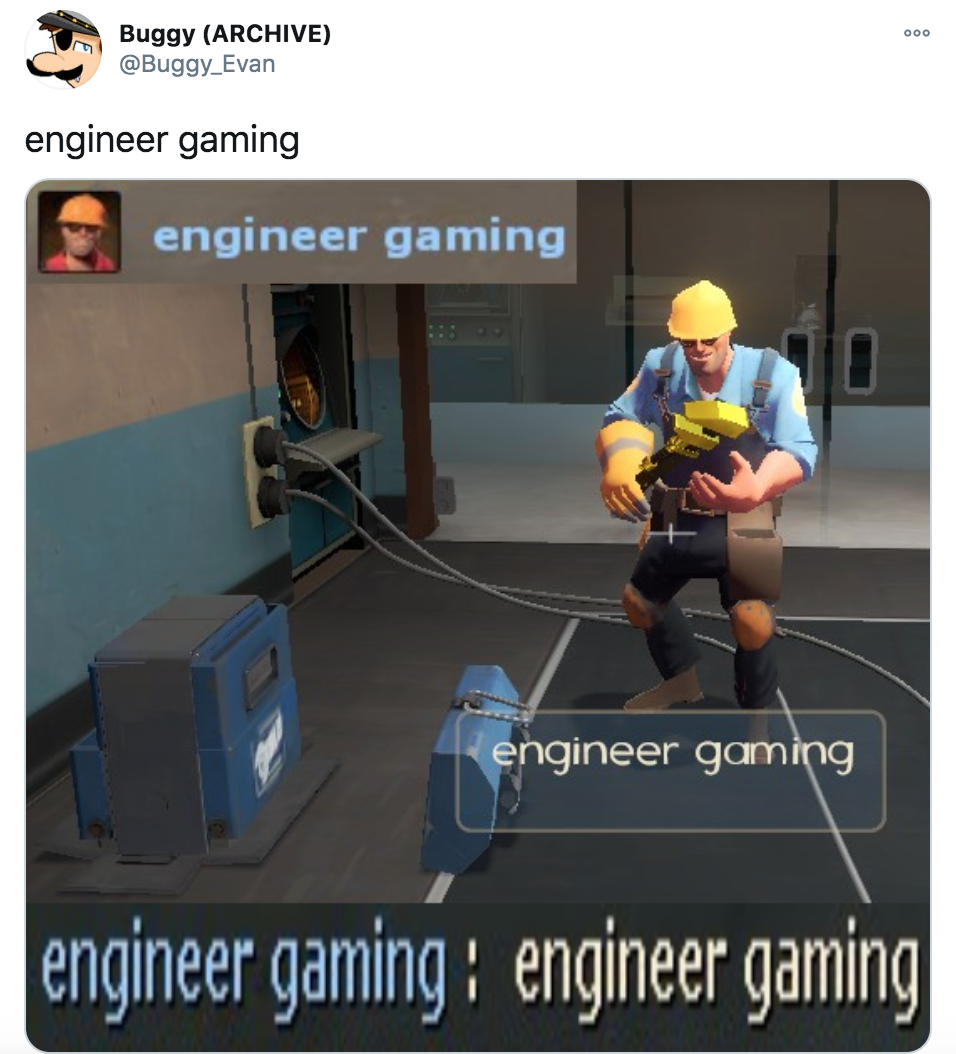
\includegraphics[scale=0.3]{img/engineer_gaming.png}
\end{figure}


I've tried to introduce it on an informal level last tutorial. Here's a more formal definition, so you can actually build your own Turing machines.

\end{frame}

\begin{frame}{What \textit{really} is a Turing machine?}
Recall: a Turing machine has a set of states (kinda like a DFA).

It reads in a symbol from the tape (at the current read-write head), consults the current state, which gives three things:
\begin{itemize}
\item A symbol to write back to the tape.
\item A new state to transition to.
\item A direction to move the read-write head.
\end{itemize}

The Turing machine takes in an input string that is prewritten on a tape, and the read-write head pointing to the first symbol in the string.
\begin{center}
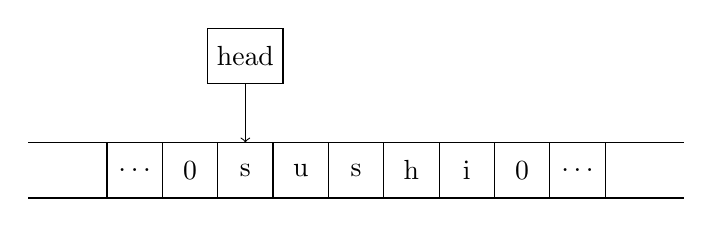
\begin{tikzpicture}[every node/.style={block},
        block/.style={minimum height=2em,minimum width=2em,outer sep=0pt,draw,rectangle,node distance=0pt}]
   \node (R1) {$\ldots$};
   \node (R2) [right=of R1] {$0$};
   \node (R3) [right=of R2] {s};
   \node (R4) [right=of R3] {u};
   \node (R5) [right=of R4] {s};
   \node (R6) [right=of R5] {h};
   \node (R7) [right=of R6] {i};
   \node (R8) [right=of R7] {$0$};
   \node (R9) [right=of R8] {$\ldots$};
   \node (HEAD) [above = 0.75cm of R3] {head};
   \draw[->] (HEAD) -- (R3);
   \draw (R1.north west) -- ++(-1cm,0) (R1.south west) -- ++ (-1cm,0);
   \draw (R9.north east) -- ++(1cm,0) (R9.south east) -- ++ (1cm,0);
\end{tikzpicture}
\end{center}
The output would just be whatever string is left on the tape at the end of execution.

\end{frame}

\begin{frame}{What \textit{really} is a Turing machine?}
Definitions (possibly from CSC236):

\vspace{4mm}

An \textbf{alphabet} is a \textit{finite} set of symbols. For example, the English alphabet is $\{a, b, \ldots, z\}$.

\vspace{2mm}

A \textbf{string} over an alphabet $\Sigma$ is a \textit{finite} sequence of symbols from $\Sigma$. For example, ``sushi'' is a string over the English alphabet. The set of all strings over an alphabet $\Sigma$ is denoted $\Sigma^*$.
\end{frame}

\begin{frame}{Formal definition}
A \textit{Turing machine} $M$ is an tuple of the form (don't blink):
$$M = (Q, \Sigma, \Gamma, \delta, q_s, F, 0).$$
Here's what each component means:
\begin{itemize}
\item $Q$ is what we referred to as the \textbf{set of states}. It's just an arbitrary (but \textit{finite}) set, so we could have $Q = \{\emojifish, \emojirice, \emojisushi\}$ if we wanted.
\item $\Sigma$ is the \textbf{input alphabet}. The Turing machine receives input strings from $\Sigma^*$.
\item $\Gamma$ is the \textbf{tape alphabet}. This represents the set of symbols that can be read and written to the tape. This satisfies $\Sigma \subseteq \Gamma$, since we better be able to read input strings.
\item $\delta$ is a weird function which will be explained later.
\end{itemize}
\end{frame}

\begin{frame}{Formal definition}
$$M = (Q, \Sigma, \Gamma, \delta, q_s, F, 0).$$
\begin{itemize}
\item $q_s$ is the \textbf{starting state}, and satisfies $q_s \in Q$.
\item $F$ is the set of \textbf{accepting states}. This satisfies $F \subseteq Q$. When we reach an accepting state, we halt and accept.
\item $0 \in \Gamma$ is the \textbf{blank symbol}. The tape is prewritten with the input string on it, and the blank symbol everywhere else.
\end{itemize}
\begin{center}
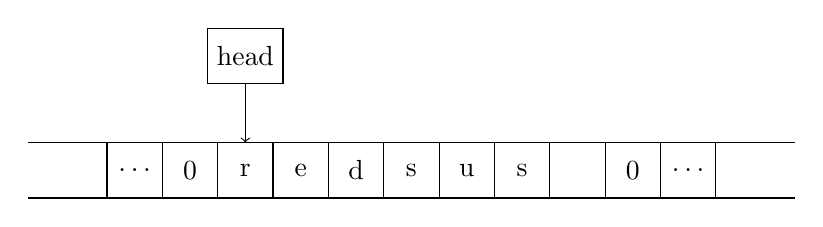
\begin{tikzpicture}[every node/.style={block},
        block/.style={minimum height=2em,minimum width=2em,outer sep=0pt,draw,rectangle,node distance=0pt}]
   \node (R1) {$\ldots$};
   \node (R2) [right=of R1] {$0$};
   \node (R3) [right=of R2] {r};
   \node (R4) [right=of R3] {e};
   \node (R5) [right=of R4] {d};
   \node (R6) [right=of R5] {s};
   \node (R7) [right=of R6] {u};
   \node (R8) [right=of R7] {s};
   \node (R9) [right=of R8] {\emojijoy};
   \node (R10) [right=of R9] {$0$};
   \node (R11) [right=of R10] {$\ldots$};
   \node (HEAD) [above = 0.75cm of R3] {head};
   \draw[->] (HEAD) -- (R3);
   \draw (R1.north west) -- ++(-1cm,0) (R1.south west) -- ++ (-1cm,0);
   \draw (R11.north east) -- ++(1cm,0) (R11.south east) -- ++ (1cm,0);
\end{tikzpicture}
\end{center}
\end{frame}

\begin{frame}{Transition function}
$$M = (Q, \Sigma, \Gamma, \delta, q_s, F, 0).$$
$\delta: (Q \times \Gamma) \to (Q \times \Gamma \times \{L, R\})$ is the \textbf{transition function}.

\vspace{2mm}

Its domain is $(Q \times \Gamma)$. The idea is that $\delta$ takes the current state and the symbol we read as input.

Its codomain is $(Q \times \Gamma \times \{L, R\})$. This means $\delta$ outputs three things: the new state to transition to, the symbol to write back, and the direction to move the read-write head.

\vspace{2mm}

Usually you will see $\delta$ defined in what is called a \textbf{transition table}.

\vspace{2mm}

Again, the Turing machine takes in an input string prewritten on the tape with blank symbols everywhere. \textit{If the Turing machine halts}, it outputs whatever is written on the tape at the time of halting.
\end{frame}

\begin{frame}{Big Chungus TM}
In this example, we attempt to design a Turing machine over the tape alphabet $\{0, \emojicarrot\}$, with input alphabet $\{\emojicarrot\}$ and blank symbol $0$. (So the possible inputs are `$\epsilon$',\footnote{$\epsilon$ is the empty string.} `\emojicarrot', ``$\emojicarrot\emojicarrot$'', ``$\emojicarrot\emojicarrot\emojicarrot$'', ...). The behaviour of this Turing machine is to output the first character of the input string, if it isn't the empty string.

\vspace{2mm}

We let $Q = \{\text{IGNORE}, \text{EAT}, \text{HALT}\}$, $\Sigma = \{\emojicarrot\}$, $\Gamma = \{0, \emojicarrot\}$, $q_s = \text{IGNORE}$, $F = \{\text{HALT}\}$, $b = 0$.
The transition table is given below:\footnote{Note that we don't need to define behaviour for halting states, since when we reach a halting state we stop.}
\begin{center}
\begin{tabular}{c|c|c}
State & $0$ & \emojicarrot\\
\hline
IGNORE & (IGNORE, $0$, R) & (EAT, $\emojicarrot$, R)\\
\hline
EAT & (HALT, $0$, R) & (EAT, $0$, R)\\
\end{tabular}
\end{center}
\end{frame}

\begin{frame}{Big Chungus TM}

\begin{center}
\begin{tabular}{c|c|c}
State & $0$ & \emojicarrot\\
\hline
IGNORE & (IGNORE, $0$, R) & (EAT, $\emojicarrot$, R)\\
\hline
EAT & (HALT, $0$, R) & (EAT, $0$, R)\\
\end{tabular}
\end{center}

On input string ``\emojicarrot\emojicarrot\emojicarrot'':

\begin{center}
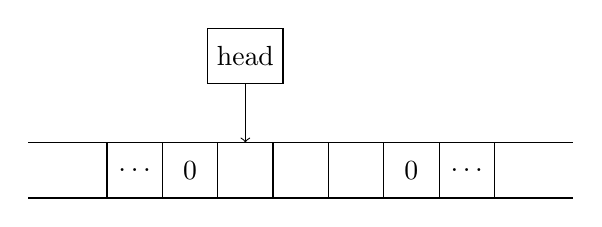
\begin{tikzpicture}[every node/.style={block},
        block/.style={minimum height=2em,minimum width=2em,outer sep=0pt,draw,rectangle,node distance=0pt}]
   \node (R1) {$\ldots$};
   \node (R2) [right=of R1] {$0$};
   \node (R3) [right=of R2] {\emojicarrot};
   \node (R4) [right=of R3] {\emojicarrot};
   \node (R5) [right=of R4] {\emojicarrot};
   \node (R6) [right=of R5] {$0$};
   \node (R7) [right=of R6] {$\ldots$};
   \node (HEAD) [above = 0.75cm of R3] {head};
   \draw[->] (HEAD) -- (R3);
   \draw (R1.north west) -- ++(-1cm,0) (R1.south west) -- ++ (-1cm,0);
   \draw (R7.north east) -- ++(1cm,0) (R7.south east) -- ++ (1cm,0);
\end{tikzpicture}
\end{center}
Current state: IGNORE (since that's our initial state)

We read in \emojicarrot. The transition table gives us $(\text{EAT}, \emojicarrot, R)$.

\end{frame}

\begin{frame}{Big Chungus TM}
\begin{center}
\begin{tabular}{c|c|c}
State & $0$ & \emojicarrot\\
\hline
IGNORE & (IGNORE, $0$, R) & (EAT, $\emojicarrot$, R)\\
\hline
EAT & (HALT, $0$, R) & (EAT, $0$, R)\\
\end{tabular}
\end{center}

\begin{center}
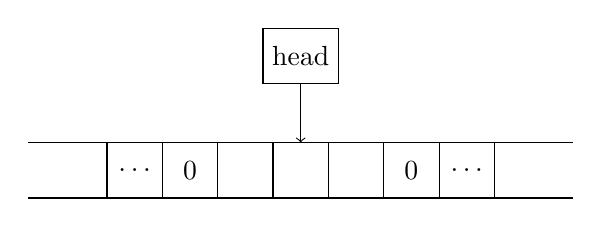
\begin{tikzpicture}[every node/.style={block},
        block/.style={minimum height=2em,minimum width=2em,outer sep=0pt,draw,rectangle,node distance=0pt}]
   \node (R1) {$\ldots$};
   \node (R2) [right=of R1] {$0$};
   \node (R3) [right=of R2] {\emojicarrot};
   \node (R4) [right=of R3] {\emojicarrot};
   \node (R5) [right=of R4] {\emojicarrot};
   \node (R6) [right=of R5] {$0$};
   \node (R7) [right=of R6] {$\ldots$};
   \node (HEAD) [above = 0.75cm of R4] {head};
   \draw[->] (HEAD) -- (R4);
   \draw (R1.north west) -- ++(-1cm,0) (R1.south west) -- ++ (-1cm,0);
   \draw (R7.north east) -- ++(1cm,0) (R7.south east) -- ++ (1cm,0);
\end{tikzpicture}
\end{center}
Current state: EAT

We read in \emojicarrot. The transition table gives us $(\text{EAT}, 0, R)$.

\end{frame}

\begin{frame}{Big Chungus TM}


\begin{center}
\begin{tabular}{c|c|c}
State & $0$ & \emojicarrot\\
\hline
IGNORE & (IGNORE, $0$, R) & (EAT, $\emojicarrot$, R)\\
\hline
EAT & (HALT, $0$, R) & (EAT, $0$, R)\\
\end{tabular}
\end{center}

\begin{center}
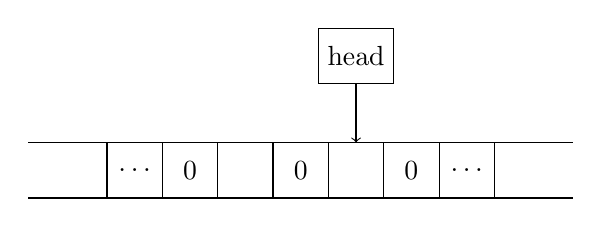
\begin{tikzpicture}[every node/.style={block},
        block/.style={minimum height=2em,minimum width=2em,outer sep=0pt,draw,rectangle,node distance=0pt}]
   \node (R1) {$\ldots$};
   \node (R2) [right=of R1] {$0$};
   \node (R3) [right=of R2] {\emojicarrot};
   \node (R4) [right=of R3] {$0$};
   \node (R5) [right=of R4] {\emojicarrot};
   \node (R6) [right=of R5] {$0$};
   \node (R7) [right=of R6] {$\ldots$};
   \node (HEAD) [above = 0.75cm of R5] {head};
   \draw[->] (HEAD) -- (R5);
   \draw (R1.north west) -- ++(-1cm,0) (R1.south west) -- ++ (-1cm,0);
   \draw (R7.north east) -- ++(1cm,0) (R7.south east) -- ++ (1cm,0);
\end{tikzpicture}
\end{center}
Current state: EAT

We read in \emojicarrot. The transition table gives us $(\text{EAT}, 0, R)$.

\end{frame}

\begin{frame}{Big Chungus TM}
\begin{center}
\begin{tabular}{c|c|c}
State & $0$ & \emojicarrot\\
\hline
IGNORE & (IGNORE, $0$, R) & (EAT, $\emojicarrot$, R)\\
\hline
EAT & (HALT, $0$, R) & (EAT, $0$, R)\\
\end{tabular}
\end{center}

\begin{center}
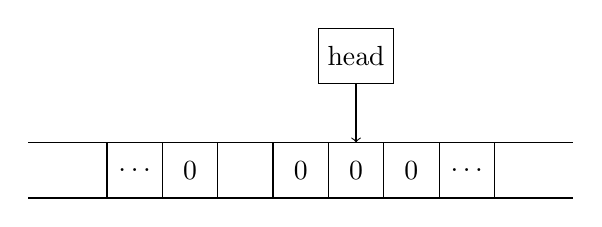
\begin{tikzpicture}[every node/.style={block},
        block/.style={minimum height=2em,minimum width=2em,outer sep=0pt,draw,rectangle,node distance=0pt}]
   \node (R1) {$\ldots$};
   \node (R2) [right=of R1] {$0$};
   \node (R3) [right=of R2] {\emojicarrot};
   \node (R4) [right=of R3] {$0$};
   \node (R5) [right=of R4] {$0$};
   \node (R6) [right=of R5] {$0$};
   \node (R7) [right=of R6] {$\ldots$};
   \node (HEAD) [above = 0.75cm of R5] {head};
   \draw[->] (HEAD) -- (R5);
   \draw (R1.north west) -- ++(-1cm,0) (R1.south west) -- ++ (-1cm,0);
   \draw (R7.north east) -- ++(1cm,0) (R7.south east) -- ++ (1cm,0);
\end{tikzpicture}
\end{center}
Current state: EAT

We read in $0$. The transition table gives us $(\text{HALT}, 0, R)$. We halt and return whatever is left on the tape, which is the string `\emojicarrot'.

\end{frame}

\begin{frame}{Now it's your turn!}
Let $\Sigma = \{0, 1\}$ be the input alphabet, $\Gamma = \{\square, 0, 1\}$ the tape alphabet, and $\square$ the blank symbol. Create a Turing machine that takes in a binary number and adds 1 to it.\footnote{You may assume the binary number starts with $1$. If this is not the case, do whatever you like.}

\vspace{2mm}

Example: Given input `10011', the Turing machine should return `10100'.

\begin{center}
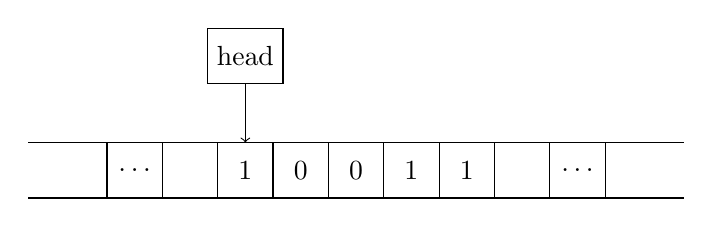
\begin{tikzpicture}[every node/.style={block},
        block/.style={minimum height=2em,minimum width=2em,outer sep=0pt,draw,rectangle,node distance=0pt}]
   \node (R1) {$\ldots$};
   \node (R2) [right=of R1] {$\square$};
   \node (R3) [right=of R2] {$1$};
   \node (R4) [right=of R3] {$0$};
   \node (R5) [right=of R4] {$0$};
   \node (R6) [right=of R5] {$1$};
   \node (R7) [right=of R6] {$1$};
   \node (R8) [right=of R7] {$\square$};
   \node (R9) [right=of R8] {$\ldots$};
   \node (HEAD) [above = 0.75cm of R3] {head};
   \draw[->] (HEAD) -- (R3);
   \draw (R1.north west) -- ++(-1cm,0) (R1.south west) -- ++ (-1cm,0);
   \draw (R9.north east) -- ++(1cm,0) (R9.south east) -- ++ (1cm,0);
\end{tikzpicture}
\end{center}

\color{red}(GO TO NEXT SLIDE: putting this here as a reminder for myself. if i don't then someone pls remind me)
\end{frame}

\begin{frame}{Now it's your turn!}
Oh yea, there's also a Turing machine simulator!

\url{https://turingmachinesimulator.com/}

\begin{figure}[h]
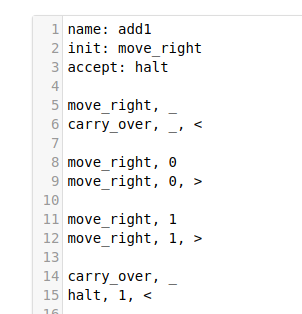
\includegraphics[scale=0.4]{img/ss1.png}

Ask me any questions on how to use it!
\end{figure}

If you're done, try building a TM that takes an input string and concatenates it to itself (example: `$10101$' goes to `$1010110101$').
\end{frame}

\begin{frame}{Your answer may differ.}
Our states will be $\{\text{MOVE}, \text{CARRY}, \text{HALT}\}$, with MOVE the initial state and HALT a final state.

\begin{center}
\begin{tabular}{c|c|c|c}
State & $\square$ & $0$ & $1$\\
\hline
MOVE & (CARRY, $\square$, L) & (MOVE, $0$, R) & (MOVE, $1$, R)\\
\hline
CARRY & (HALT, $1$, L) & (HALT, $1$, L) & (CARRY, $0$, L)\\
\end{tabular}
\end{center}
Current state: MOVE 

\begin{center}
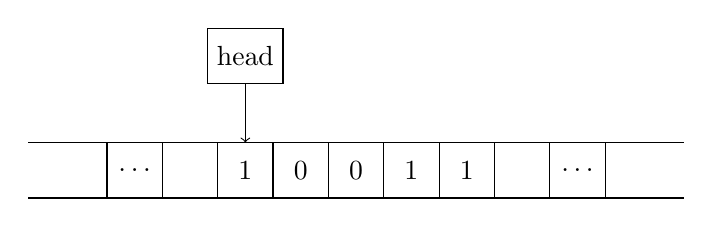
\begin{tikzpicture}[every node/.style={block},
        block/.style={minimum height=2em,minimum width=2em,outer sep=0pt,draw,rectangle,node distance=0pt}]
   \node (R1) {$\ldots$};
   \node (R2) [right=of R1] {$\square$};
   \node (R3) [right=of R2] {$1$};
   \node (R4) [right=of R3] {$0$};
   \node (R5) [right=of R4] {$0$};
   \node (R6) [right=of R5] {$1$};
   \node (R7) [right=of R6] {$1$};
   \node (R8) [right=of R7] {$\square$};
   \node (R9) [right=of R8] {$\ldots$};
   \node (HEAD) [above = 0.75cm of R3] {head};
   \draw[->] (HEAD) -- (R3);
   \draw (R1.north west) -- ++(-1cm,0) (R1.south west) -- ++ (-1cm,0);
   \draw (R9.north east) -- ++(1cm,0) (R9.south east) -- ++ (1cm,0);
\end{tikzpicture}
\end{center}

We keep going right until we encounter $\square$.

\end{frame}

\begin{frame}{Your answer may differ.}
\begin{center}
\begin{tabular}{c|c|c|c}
State & $\square$ & $0$ & $1$\\
\hline
MOVE & (CARRY, $\square$, L) & (MOVE, $0$, R) & (MOVE, $1$, R)\\
\hline
CARRY & (HALT, $1$, L) & (HALT, $1$, L) & (CARRY, $0$, L)\\
\end{tabular}
\end{center}
Current state: MOVE 

\begin{center}
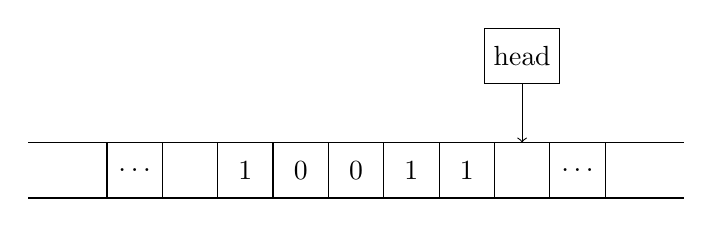
\begin{tikzpicture}[every node/.style={block},
        block/.style={minimum height=2em,minimum width=2em,outer sep=0pt,draw,rectangle,node distance=0pt}]
   \node (R1) {$\ldots$};
   \node (R2) [right=of R1] {$\square$};
   \node (R3) [right=of R2] {$1$};
   \node (R4) [right=of R3] {$0$};
   \node (R5) [right=of R4] {$0$};
   \node (R6) [right=of R5] {$1$};
   \node (R7) [right=of R6] {$1$};
   \node (R8) [right=of R7] {$\square$};
   \node (R9) [right=of R8] {$\ldots$};
   \node (HEAD) [above = 0.75cm of R8] {head};
   \draw[->] (HEAD) -- (R8);
   \draw (R1.north west) -- ++(-1cm,0) (R1.south west) -- ++ (-1cm,0);
   \draw (R9.north east) -- ++(1cm,0) (R9.south east) -- ++ (1cm,0);
\end{tikzpicture}
\end{center}

We've encountered $\square$. Transition to state CARRY, write $\square$, and go left.

\end{frame}

\begin{frame}{Your answer may differ.}
\begin{center}
\begin{tabular}{c|c|c|c}
State & $\square$ & $0$ & $1$\\
\hline
MOVE & (CARRY, $\square$, L) & (MOVE, $0$, R) & (MOVE, $1$, R)\\
\hline
CARRY & (HALT, $1$, L) & (HALT, $1$, L) & (CARRY, $0$, L)\\
\end{tabular}
\end{center}
Current state: CARRY 

\begin{center}
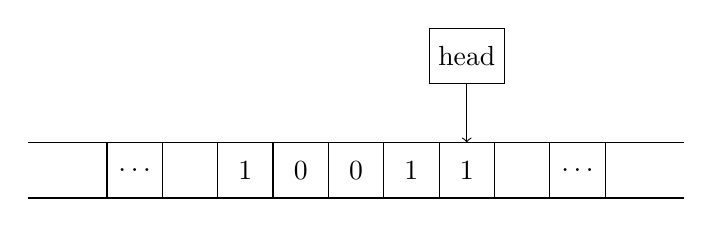
\begin{tikzpicture}[every node/.style={block},
        block/.style={minimum height=2em,minimum width=2em,outer sep=0pt,draw,rectangle,node distance=0pt}]
   \node (R1) {$\ldots$};
   \node (R2) [right=of R1] {$\square$};
   \node (R3) [right=of R2] {$1$};
   \node (R4) [right=of R3] {$0$};
   \node (R5) [right=of R4] {$0$};
   \node (R6) [right=of R5] {$1$};
   \node (R7) [right=of R6] {$1$};
   \node (R8) [right=of R7] {$\square$};
   \node (R9) [right=of R8] {$\ldots$};
   \node (HEAD) [above = 0.75cm of R7] {head};
   \draw[->] (HEAD) -- (R7);
   \draw (R1.north west) -- ++(-1cm,0) (R1.south west) -- ++ (-1cm,0);
   \draw (R9.north east) -- ++(1cm,0) (R9.south east) -- ++ (1cm,0);
\end{tikzpicture}
\end{center}

Transition to state CARRY (i mean, we're already in state CARRY), write $0$, and move left.

\end{frame}

\begin{frame}{Your answer may differ.}
\begin{center}
\begin{tabular}{c|c|c|c}
State & $\square$ & $0$ & $1$\\
\hline
MOVE & (CARRY, $\square$, L) & (MOVE, $0$, R) & (MOVE, $1$, R)\\
\hline
CARRY & (HALT, $1$, L) & (HALT, $1$, L) & (CARRY, $0$, L)\\
\end{tabular}
\end{center}
Current state: CARRY 

\begin{center}
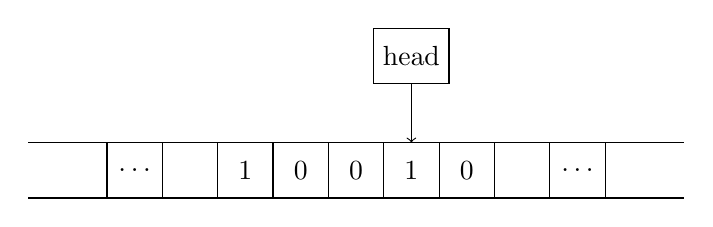
\begin{tikzpicture}[every node/.style={block},
        block/.style={minimum height=2em,minimum width=2em,outer sep=0pt,draw,rectangle,node distance=0pt}]
   \node (R1) {$\ldots$};
   \node (R2) [right=of R1] {$\square$};
   \node (R3) [right=of R2] {$1$};
   \node (R4) [right=of R3] {$0$};
   \node (R5) [right=of R4] {$0$};
   \node (R6) [right=of R5] {$1$};
   \node (R7) [right=of R6] {$0$};
   \node (R8) [right=of R7] {$\square$};
   \node (R9) [right=of R8] {$\ldots$};
   \node (HEAD) [above = 0.75cm of R6] {head};
   \draw[->] (HEAD) -- (R6);
   \draw (R1.north west) -- ++(-1cm,0) (R1.south west) -- ++ (-1cm,0);
   \draw (R9.north east) -- ++(1cm,0) (R9.south east) -- ++ (1cm,0);
\end{tikzpicture}
\end{center}

Transition to state CARRY (i mean, we're already in state CARRY), write $0$, and move left.

\end{frame}

\begin{frame}{Your answer may differ.}
\begin{center}
\begin{tabular}{c|c|c|c}
State & $\square$ & $0$ & $1$\\
\hline
MOVE & (CARRY, $\square$, L) & (MOVE, $0$, R) & (MOVE, $1$, R)\\
\hline
CARRY & (HALT, $1$, L) & (HALT, $1$, L) & (CARRY, $0$, L)\\
\end{tabular}
\end{center}
Current state: CARRY 

\begin{center}
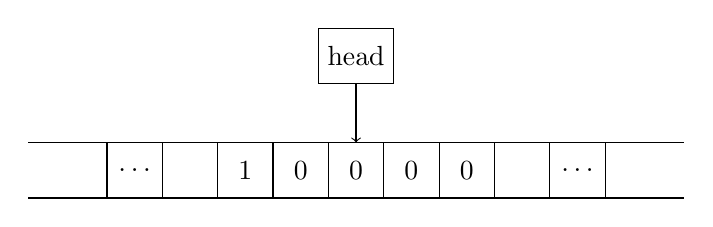
\begin{tikzpicture}[every node/.style={block},
        block/.style={minimum height=2em,minimum width=2em,outer sep=0pt,draw,rectangle,node distance=0pt}]
   \node (R1) {$\ldots$};
   \node (R2) [right=of R1] {$\square$};
   \node (R3) [right=of R2] {$1$};
   \node (R4) [right=of R3] {$0$};
   \node (R5) [right=of R4] {$0$};
   \node (R6) [right=of R5] {$0$};
   \node (R7) [right=of R6] {$0$};
   \node (R8) [right=of R7] {$\square$};
   \node (R9) [right=of R8] {$\ldots$};
   \node (HEAD) [above = 0.75cm of R5] {head};
   \draw[->] (HEAD) -- (R5);
   \draw (R1.north west) -- ++(-1cm,0) (R1.south west) -- ++ (-1cm,0);
   \draw (R9.north east) -- ++(1cm,0) (R9.south east) -- ++ (1cm,0);
\end{tikzpicture}
\end{center}

Transition to state HALT, write $1$, and move left.

\end{frame}

\begin{frame}{Your answer may differ.}






\begin{center}
\begin{tabular}{c|c|c|c}
State & $\square$ & $0$ & $1$\\
\hline
MOVE & (CARRY, $\square$, L) & (MOVE, $0$, R) & (MOVE, $1$, R)\\
\hline
CARRY & (HALT, $1$, L) & (HALT, $1$, L) & (CARRY, $0$, L)\\
\end{tabular}
\end{center}
Current state: HALT 

\begin{center}
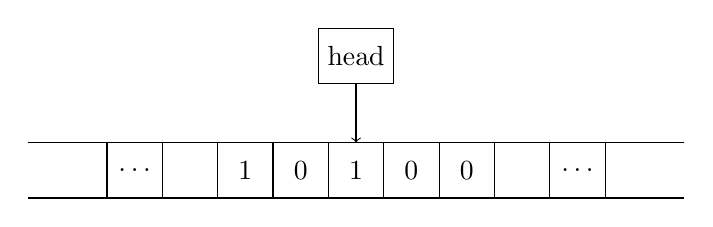
\begin{tikzpicture}[every node/.style={block},
        block/.style={minimum height=2em,minimum width=2em,outer sep=0pt,draw,rectangle,node distance=0pt}]
   \node (R1) {$\ldots$};
   \node (R2) [right=of R1] {$\square$};
   \node (R3) [right=of R2] {$1$};
   \node (R4) [right=of R3] {$0$};
   \node (R5) [right=of R4] {$1$};
   \node (R6) [right=of R5] {$0$};
   \node (R7) [right=of R6] {$0$};
   \node (R8) [right=of R7] {$\square$};
   \node (R9) [right=of R8] {$\ldots$};
   \node (HEAD) [above = 0.75cm of R5] {head};
   \draw[->] (HEAD) -- (R5);
   \draw (R1.north west) -- ++(-1cm,0) (R1.south west) -- ++ (-1cm,0);
   \draw (R9.north east) -- ++(1cm,0) (R9.south east) -- ++ (1cm,0);
\end{tikzpicture}
\end{center}

Since HALT is a final state, return `10100'.

\end{frame}

\begin{frame}{The power of Turing machines}
\textit{Everything your computer can do can also be done by a Turing machine.}

\vspace{2mm}

We won't prove the above statement, just believe in it.\footnote{Big Chungus demands you to believe in this statement, and erase any doubt of it in your head.} But since computers can simulate Turing machines,\footnote{sponsored by \url{https://turingmachinesimulator.com/}} \textit{there exists a Turing machine that simulates Turing machines}. This Turing machine simulating Turing machine is called the \textbf{universal Turing machine}.
\end{frame}

\begin{frame}{Acceptance and refusal (from cs post ;-;)}
Sometimes we want Turing machines to ``accept'' and ``reject'' strings, just like DFAs.\footnote{In this convention, the Turing machine is a function that takes in a string, and outputs a boolean value (assuming it halts).}

Remember $F$, the set of final states in the definition of a Turing machine? Instead of that, we add two additional states to $Q$, called $q_\text{accept}$ and $q_\text{reject}$. 

Instead of transitioning to halting states, we transition to either $q_\text{accept}$ or $q_\text{reject}$, and halt. 

We say a TM \textbf{accepts} a string $s$ if on input $s$, it halts and ends in state $q_\text{accept}$. We say a TM \textbf{rejects} $s$ if on input $s$, it halts and ends in $q_\text{reject}$. 

\vspace{2mm}

Note a TM may still loop on input $s$. In this case it neither accepts or rejects, and we say it \textbf{loops} on $s$. A TM \textbf{halts} on $s$ if it either accepts or rejects $s$.
\end{frame}

\begin{frame}{Quick exercise}
Give an example of a Turing machine that doesn't halt on any input.
\begin{figure}[h]
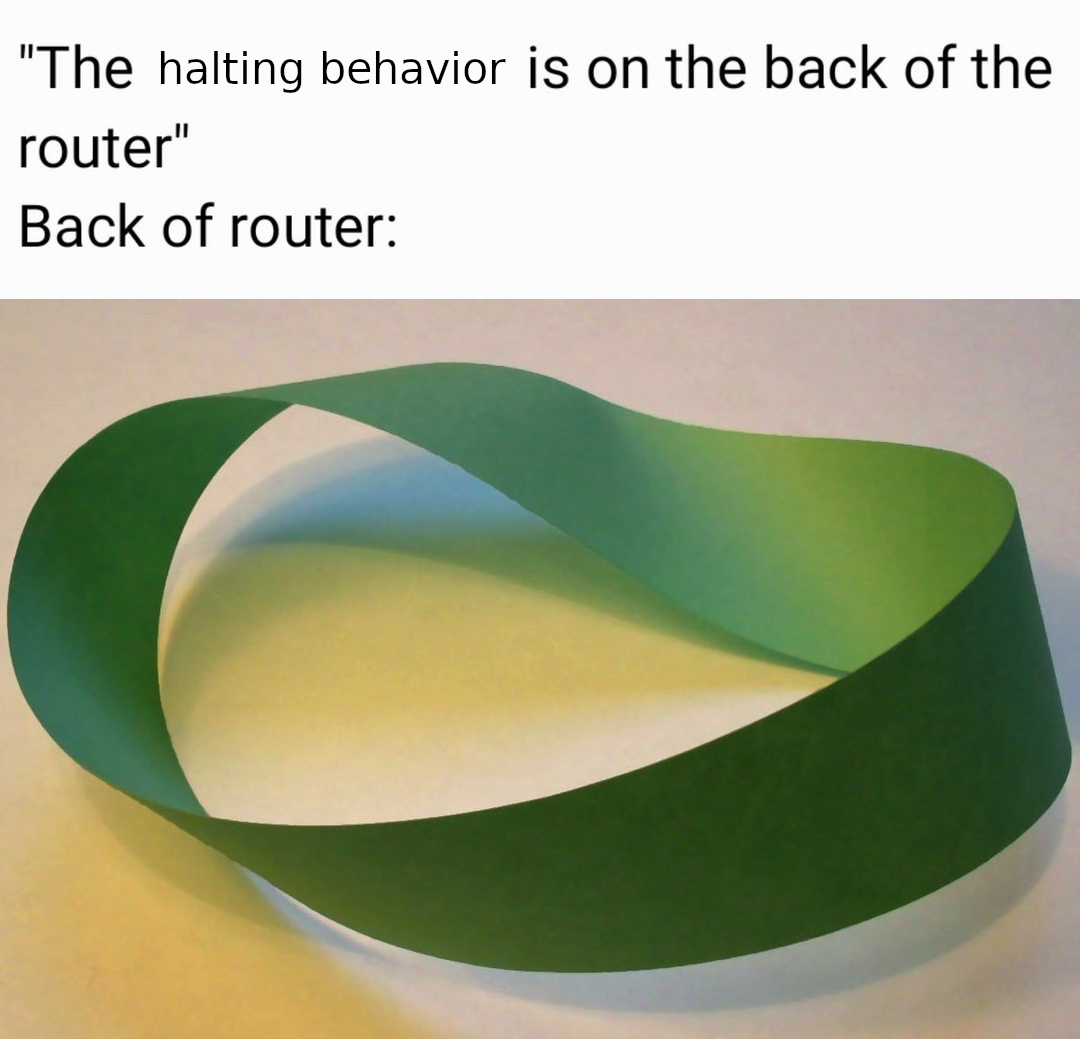
\includegraphics[scale=0.7]{img/halting.jpg}
\end{figure}
\end{frame}

\begin{frame}{Acceptance and refusal (from cs post ;-;)}
Example: we can modify the add-1 Turing machine earlier to reject inputs not starting with $1$, and otherwise add 1 to the input and accept.

\vspace{2mm}

Original: set of states was $\{\text{MOVE}, \text{CARRY}, \text{HALT}\}$, initial state MOVE.
\begin{center}
\begin{tabular}{c|c|c|c}
State & $\square$ & $0$ & $1$\\
\hline
MOVE & (CARRY, $\square$, L) & (MOVE, $0$, R) & (MOVE, $1$, R)\\
\hline
CARRY & (HALT, $1$, L) & (HALT, $1$, L) & (CARRY, $0$, L)\\
\end{tabular}
\end{center}

\vspace{2mm}

Modified: $\{\text{START}, \text{MOVE}, \text{CARRY}, q_\text{accept}, q_\text{reject}\}$, initial state START.
\begin{center}
\begin{tabular}{c|c|c|c}
State & $\square$ & $0$ & $1$\\
\hline
START & ($q_\text{reject}$, $\square$, R) & ($q_\text{reject}$, $\square$, R) & (MOVE, $1$, R)\\
\hline
MOVE & (CARRY, $\square$, L) & (MOVE, $0$, R) & (MOVE, $1$, R)\\
\hline
CARRY & ($q_\text{accept}$, $1$, L) & ($q_\text{accept}$, $1$, L) & (CARRY, $0$, L)\\
\end{tabular}
\end{center}
\end{frame}

\begin{frame}{Computable and listable Sets}
A \textbf{language} over an alphabet $\Sigma$ is a (possibly infinite) collection of strings from $\Sigma^*$. For example, the set of English words is a language over the English alphabet.

\vspace{2mm}

Given a Turing machine $M$ with input alphabet $\Sigma$, we define $L(M)$ (the \textbf{language} of $M$) to be the following language over $\Sigma$:
$$L(M) = \{s \in \Sigma^*: \text{$M$ accepts $s$}\}.$$
\end{frame}

\begin{frame}{Computable and listable Sets}
A language $\mathcal L$ over $\Sigma$ is \textbf{listable} if there exists a Turing machine $M$ with input alphabet $\Sigma$ such that $\mathcal L = L(M)$.\footnote{The definition of ``listable'' given here is equivalent to the Turing-machine definition from the first lecture, which is equivalent to ``computably enumerable'' from the second lecture.}

\vspace{2mm}

A language $\mathcal L$ over $\Sigma$ is \textbf{decidable} if there exists a Turing machine $M$ with input alphabet $\Sigma$ such that $\mathcal L = L(M)$, \textit{and $M$ halts on all input strings}.\footnote{Same here. A Turing machine that halts on all inputs is called a \textbf{decider}.}

The ``hierarchy'' of languages goes like this:
$$\text{Regular Languages} \subset \text{Decidable L.} \subset \text{Listable L.} \subset \text{All L.}$$
If you don't remember regular languages\footnote{Every regular language is decidable. Why? We can simulate a DFA on a computer, so we can simulate a DFA on a Turing machine. DFAs always halt, so the DFA simulator always halts given any input.} from CSC236, don't worry.

\end{frame}

\begin{frame}{Computable and listable Sets}
One more thing to note: each Turing machine can be encoded in an ASCII string.\footnote{again, sponsored by \url{https://turingmachinesimulator.com/}}

\begin{figure}[h]
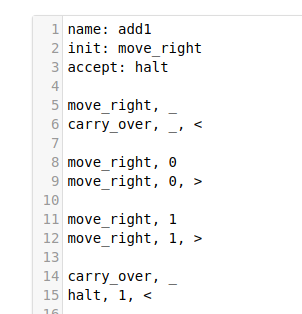
\includegraphics[scale=0.4]{img/ss1.png}
\end{figure}

So if $\Sigma$ is the ASCII alphabet, then ``the set of valid Turing machine encodings'' is a language over $\Sigma$.

\end{frame}

\begin{frame}{Halting problem}
Now we can prove the existence of an undecidable but listable language. This language is called the \textbf{halting problem}, denoted by HP.\footnote{Formally I have to declare the alphabet first, but this is usually omitted if the alphabet is not relevant. I'll just choose the alphabet to be the ASCII characters.}

$$\text{HP} = \{Mw: \text{$M$ is a Turing machine that halts on $w$}\}.$$

Why is this language listable? The language of the following ``Turing machine'' $M'$ is precisely $\text{HP}$:\footnote{Remember, whatever a computer can do, so can a Turing machine.}
\begin{align*}
M'(s): & \quad \text{if $s$ is of the form $Mw$:}\\
& \quad \quad \text{Simulate $M$ on $w$}\\
& \quad \quad \text{accept}\\
& \quad \text{reject}
\end{align*}
Note that this isn't guaranteed to halt: in the case $M$ doesn't halt on $w$, the third line will take forever. So this doesn't show HP is decidable.
\end{frame}

\begin{frame}{Halting problem}
Why isn't HP decidable? We prove by contradiction. Suppose HP is decidable (so there exists a Turing machine $D$ such that $L(D) = \text{HP}$ and $D$ halts on all inputs).

\vspace{2mm}

Construct the following Turing machine $P$:
\begin{align*}
P(s): & \quad \text{if $s$ is a Turing machine $M$:}\\
& \quad \quad \text{If $D$ accepts $MM$:}\\
& \quad \quad \quad \text{loop}\\
& \quad \text{accept}
\end{align*}

Notice $P$ never rejects, so it either accepts or loops given any input. Consider $P(P)$.

\end{frame}

\begin{frame}{Halting problem}
\begin{align*}
P(s): & \quad \text{if $s$ is a Turing machine $M$:}\\
& \quad \quad \text{If $D$ accepts $MM$:}\\
& \quad \quad \quad \text{loop}\\
& \quad \text{accept}
\end{align*}
If $P(P)$ accepts, then $D$ must have rejected $PP$. But then that means $P(P)$ doesn't halt, so $P$ can't have accepted $P$.

\vspace{2mm}

If $P(P)$ loops, then $D$ must have accepted $PP$. But by definition that means $P(P)$ halts, so $P(P)$ can't loop. 

\vspace{2mm}

We conclude no such $D$ exists, meaning $\text{HP}$ is undecidable.

\end{frame}

\begin{frame}{Okay but what's the practical use?}

None that I know of. Hey, we mentioned no programming in this course!

\vspace{2mm}


Anyway, bye! If you wanna challenge yourself, try reading the lecture slides from this week again, but actually understanding what's going on by relating it to what I presented here.

\end{frame}

\begin{frame}{License}

  \begin{block}{Get the source of this theme and the demo presentation from}

  \begin{center}\url{http://github.com/famuvie/beamerthemesimple}\end{center}

  \end{block}
  
  The theme \emph{itself} is licensed under a
  \href{http://creativecommons.org/licenses/by-sa/4.0/}{Creative Commons
  Attribution-ShareAlike 4.0 International License}.

  \begin{center}\ccbysa\end{center}

\end{frame}

\end{document}